% !TeX program = lualatex
% !TeX encoding = utf8
% !TeX spellcheck = uk_UA

\documentclass{article}
\usepackage{tikz, pgfplots}


\begin{document}
\begin{center}
	\begin{minipage}{0.75\linewidth}
		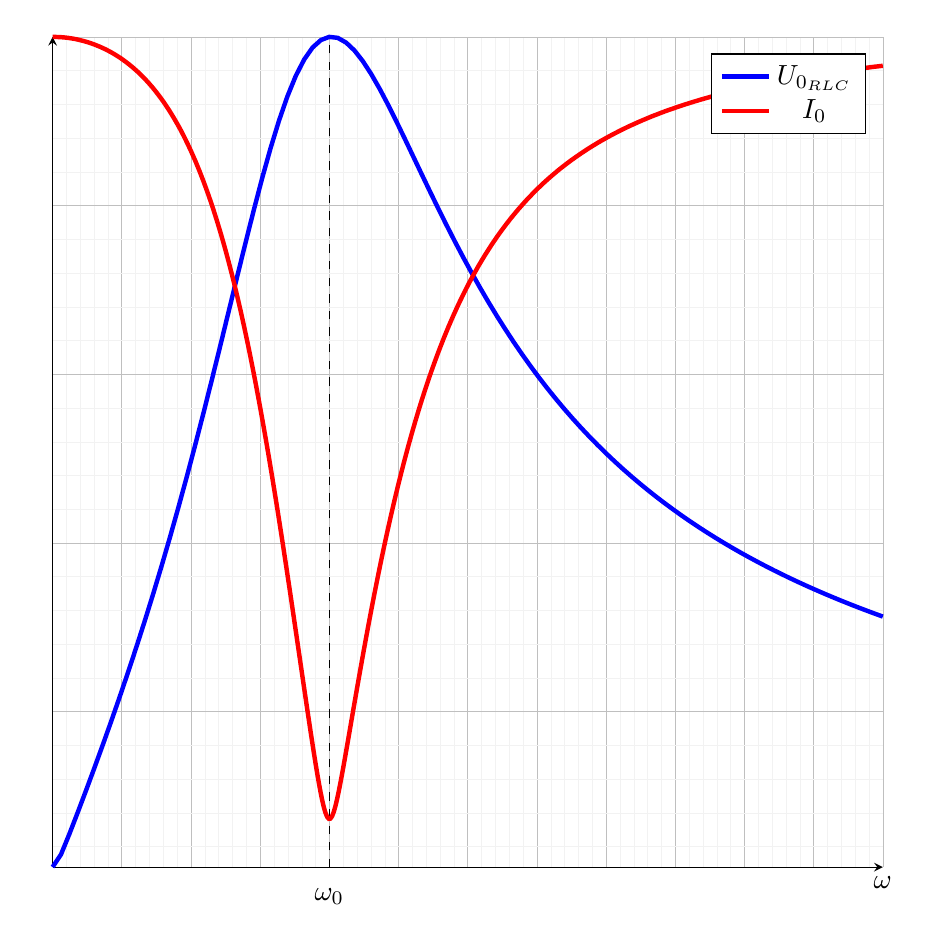
\begin{tikzpicture}[/pgf/foreach/parse=true,
				declare function = {
						L = 2e-0;
						C = 1e-3;
						R = 1e3;
						RI = 50;
						RL = 0.8;
						Ri = 5 ;
						E = 10;
						omegares = 1/sqrt(L*C);
						a(\x) = 1/R + RL/(RL^2 + \x^2*L^2);
						b(\x) = \x*C - \x*L/(RL^2 + \x^2*L^2);
						c(\x) = (RI + Ri) + a(\x)/(a(\x)^2 + b(\x)^2);
						d(\x) =  b(\x)/(a(\x)^2 + b(\x)^2);
						g(\x) = c(\x)^2 + d(\x)^2;
						I(\x) = E/sqrt(g(\x));
						Imin = I(omegares);
						U(\x) = E*sqrt( (1- (Ri+ RI)*c(\x)/g(\x))^2 + ((Ri+ RI)*d(\x)/g(\x))^2 );
						Umax = U(omegares);
						I2(\x) = U(\x)*sqrt(a(\x)^2 + b(\x)^2);
					},
			]
			\begin{axis}[clip = false,
					% === Налаштування сітки ===
					grid = both,
					grid style={line width=.1pt, draw=gray!10},
					major grid style={line width=.2pt,draw=gray!50},
					minor tick num = 4,
					minor grid style = {line width=.1pt,draw=gray!10},
					% === Налаштування положення координатних осей ===
					axis lines = middle,
					axis line style={-stealth},
					% === Підпис координатних осей ===
					%				xticklabels={},
					xlabel={$\omega$},
					%				ylabel={$\frac{U_{0_{RLC}}}{U_{0_{\max}}}$},
					% === Положення підпису координатних осей ===
					ylabel style={left},
					xlabel style={below},
					extra tick style={% changes for all extra ticks
							tick align=outside,
							major grid style={dashed,draw=black}
						},
					extra x tick style={
							major tick style={
								},
							tick label style={
									/pgf/number format/.cd, fixed, fixed zerofill,
									precision=2,
								}
						},
					xtick style={draw=none},
					ytick style={draw=none},
					xticklabels={},
					yticklabels={},
					extra x ticks={omegares},
					extra x tick labels={$\omega_0$},
					%				extra y ticks={(E - I(0)*(Ri + RI))/Umax},
					%				extra y tick labels={$\frac{\mathcal{E} - I(0)\cdot R_i}{U_{\max}}$},
					% === Вибір підписів шкали для відображення ===
					xtick = {0,0.25*omegares,...,3*omegares},
					ytick = {0,0.2,...,1},
					% === Налаштування мінімальних та максимальних значень координат ===
					xmin = 0*omegares,
					xmax =  3*omegares,
					ymin = {(E - I(0)*(Ri + RI))/Umax},
					ymax =  1,
					% === Налаштування розміру графіка ===
					width=1\linewidth,
					height=1\linewidth,
				]

				\addplot [ultra thick,samples = 100, domain=0:3*omegares, blue] {U(x)/Umax};
				\addplot [ultra thick,samples = 500, domain=0:3*omegares, red] {I(x)/I(0)};


				\legend{$U_{0_{RLC}}$, $I_0$,$I2$}	
			\end{axis}
		\end{tikzpicture}
%		\captionof{figure}{Амплітудно-частотна характеристика напруги та струму в паралельному колі}
		\label{plt:P-AFC-URLC}
	\end{minipage}
\end{center}
\end{document}

